\documentclass[12pt,a4paper]{article}

% ── Packages ──────────────────────────────────────────────────────────────────
\usepackage[T1]{fontenc}
\usepackage[utf8]{inputenc}
\usepackage{lmodern}
\usepackage[margin=2.5cm]{geometry}
\usepackage{graphicx}
\usepackage{xcolor}
\usepackage{hyperref}
\usepackage{booktabs}
\usepackage{tabularx}
\usepackage{array}
\usepackage{enumitem}
\usepackage{listings}
\usepackage{caption}
\usepackage{subcaption}
\usepackage{fancyhdr}
\usepackage{titlesec}
\usepackage{tikz}
\usepackage{mdframed}
\usepackage{amsmath}
\usepackage{float}
\usepackage{microtype}

% ── Colours ───────────────────────────────────────────────────────────────────
\definecolor{etOrange}{RGB}{249,115,22}
\definecolor{etDark}{RGB}{15,23,42}
\definecolor{etSlate}{RGB}{51,65,85}
\definecolor{etMuted}{RGB}{100,116,139}
\definecolor{codeGray}{RGB}{248,249,250}
\definecolor{codeBorder}{RGB}{222,226,230}

% ── Hyperlinks ────────────────────────────────────────────────────────────────
\hypersetup{
    colorlinks=true,
    linkcolor=etOrange,
    urlcolor=etOrange,
    citecolor=etOrange,
    pdftitle={ET AI Concierge — Technical Report},
    pdfauthor={Nimish},
}

% ── Section Styling ───────────────────────────────────────────────────────────
\titleformat{\section}
  {\large\bfseries\color{etDark}}
  {\thesection.}{0.5em}{}[\color{etOrange}\titlerule]

\titleformat{\subsection}
  {\normalsize\bfseries\color{etSlate}}
  {\thesubsection.}{0.5em}{}

\titleformat{\subsubsection}
  {\normalsize\itshape\color{etMuted}}
  {\thesubsubsection.}{0.5em}{}

% ── Code Style ────────────────────────────────────────────────────────────────
\lstset{
    backgroundcolor=\color{codeGray},
    basicstyle=\small\ttfamily,
    breaklines=true,
    frame=single,
    rulecolor=\color{codeBorder},
    keywordstyle=\color{etOrange}\bfseries,
    stringstyle=\color{etSlate},
    commentstyle=\color{etMuted}\itshape,
    numbers=left,
    numberstyle=\tiny\color{etMuted},
    numbersep=5pt,
    showstringspaces=false,
    tabsize=4,
    captionpos=b,
}

% ── Header / Footer ───────────────────────────────────────────────────────────
\pagestyle{fancy}
\fancyhf{}
\fancyhead[L]{\small\textcolor{etMuted}{ET AI Concierge}}
\fancyhead[R]{\small\textcolor{etMuted}{Technical Report}}
\fancyfoot[C]{\small\textcolor{etMuted}{\thepage}}
\renewcommand{\headrulewidth}{0.4pt}

% ── Callout Box ───────────────────────────────────────────────────────────────
\newmdenv[
  backgroundcolor=etOrange!8,
  linecolor=etOrange,
  linewidth=2pt,
  leftline=true, rightline=false, topline=false, bottomline=false,
  innerleftmargin=10pt,
  innertopmargin=6pt,
  innerbottommargin=6pt,
]{highlight}

% ══════════════════════════════════════════════════════════════════════════════
\begin{document}

% ── Title Page ────────────────────────────────────────────────────────────────
\begin{titlepage}
\centering
\vspace*{2cm}

{\Huge\bfseries\color{etOrange} ET AI Concierge}\\[0.5em]
{\Large\color{etSlate} Technical Design \& Implementation Report}\\[2em]

\rule{12cm}{1.5pt}\\[1.5em]

{\large\textbf{Problem Statement 7} — AI Concierge for Economic Times}\\[1em]
{\normalsize\color{etMuted}
Economic Times Hackathon\\
\textit{Submitted by: Nimish}\\
}\\[1em]

\rule{12cm}{0.5pt}\\[2em]

{\normalsize
\begin{tabular}{ll}
\textbf{Backend}   & FastAPI (Python 3.11) \\
\textbf{Frontend}  & Next.js 14 (App Router) \\
\textbf{LLM}       & Groq \texttt{llama-3.3-70b-versatile} \\
\textbf{Vector DB} & Weaviate (Cloud / Local) \\
\textbf{Embeddings}& sentence-transformers \texttt{all-MiniLM-L6-v2} \\
\textbf{Repository}& \url{https://github.com/nimish1402/ET-Concierge} \\
\end{tabular}
}

\vfill
{\small\textcolor{etMuted}{March 2026}}
\end{titlepage}

% ── Table of Contents ─────────────────────────────────────────────────────────
\tableofcontents
\newpage

% ══════════════════════════════════════════════════════════════════════════════
\section{Problem Statement}

\subsection{Background}

Economic Times (ET) has built one of India's most comprehensive financial ecosystems, spanning:

\begin{itemize}[noitemsep]
  \item \textbf{ET Prime} — Premium news and analysis
  \item \textbf{ET Markets} — Real-time stock portfolio tracking
  \item \textbf{ET Money} — Mutual funds, SIPs, and tax-saving investments
  \item \textbf{Masterclasses} — Financial education programs
  \item \textbf{Corporate Events \& Wealth Summits} — Networking and expert insights
  \item \textbf{Financial Services Partnerships} — Credit cards, loans, insurance
\end{itemize}

Despite this breadth, the core challenge is stark:

\begin{highlight}
\textbf{Most users discover only 10\% of what ET offers.} There is no intelligent layer that understands who the user is and actively guides them to the full ET ecosystem.
\end{highlight}

\subsection{Official Problem Statement}

The problem statement (PS-7) challenges participants to build an \textbf{AI Concierge} that:

\begin{enumerate}[noitemsep]
  \item Understands who the user is in one conversation
  \item Becomes a personal guide to everything ET can do for them
\end{enumerate}

Specifically, the problem identifies four solution areas:

\begin{table}[H]
\centering
\caption{Problem Statement Solution Areas}
\begin{tabularx}{\textwidth}{lX}
\toprule
\textbf{Component} & \textbf{Description} \\
\midrule
ET Welcome Concierge & AI voice/chat agent greets users with smart 3-minute profiling, maps them to ET products, creates personalised onboarding path \\
\addlinespace
Financial Life Navigator & Deep conversational AI that understands the user's complete financial life, identifies portfolio gaps, goals, and immediate needs \\
\addlinespace
Cross-Sell Engine & AI across all ET touchpoints proactively identifying cross-sell/upsell opportunities based on user behaviour and profile \\
\addlinespace
Services Marketplace Agent & Conversational AI acting as a concierge for credit cards, loans, insurance, and wealth management via ET partnerships \\
\bottomrule
\end{tabularx}
\end{table}

% ══════════════════════════════════════════════════════════════════════════════
\section{Our Solution}

\subsection{Overview}

We implemented a full-stack, production-ready AI concierge platform that addresses \textbf{all four} solution areas using only free-tier and open-source tools.

\begin{highlight}
\textbf{Key Principle:} Zero paid API costs. The entire system runs on Groq's free tier, Weaviate's free sandbox, and a local embedding model (\texttt{all-MiniLM-L6-v2}).
\end{highlight}

\subsection{Solution Components}

\subsubsection{ET Welcome Concierge}
A stateless, chat-based onboarding system powered by Groq's \texttt{llama-3.3-70b-versatile}. The LLM asks 5–7 targeted questions and automatically detects when it has sufficient information. It then self-extracts a structured financial persona JSON:

\begin{lstlisting}[language=Python, caption=Extracted Profile Schema]
{
  "persona": "student | young_professional | mid_career | ...",
  "risk_level": "conservative | moderate | aggressive",
  "goals": ["list of stated financial goals"],
  "interests": ["sip", "mutual funds", "tax saving", ...],
  "recommended_products": ["ET Money SIP", "ET Markets", ...]
}
\end{lstlisting}

\subsubsection{Financial Life Navigator (RAG Pipeline)}
After onboarding, subsequent user queries enter the \textbf{Retrieval-Augmented Generation} pipeline:

\begin{enumerate}[noitemsep]
  \item User query is embedded using \texttt{all-MiniLM-L6-v2} (local, no API call)
  \item Weaviate performs \texttt{near\_vector} similarity search across \texttt{FinancialContent} and \texttt{ETProduct} collections
  \item Top-$k$ context chunks are passed to Groq alongside the user profile
  \item Groq returns a personalised, context-grounded answer
\end{enumerate}

\subsubsection{Cross-Sell Recommendation Engine}
A rule-based scoring engine evaluates every product in the ET catalog against the user's profile and behaviour:

\begin{equation}
\text{score} = W_{\text{interest}} + W_{\text{persona/risk}} + W_{\text{behaviour}}
\end{equation}

Where:
\begin{align*}
W_{\text{interest}}         &\in [0, 40] \quad \text{(tag overlap between user interests and product tags)} \\
W_{\text{persona/risk}}     &\in [0, 30] \quad \text{(persona match: +20, risk level match: +10)} \\
W_{\text{behaviour}}        &\in [0, 30] \quad \text{(click: +5, search: +7, view: +3 per event)}
\end{align*}

Top-5 products are ranked and presented on the dashboard with AI-generated explanations.

\subsubsection{Services Marketplace Agent}
A curated catalog of 8 ET financial products (SIP, ELSS, NPS, insurance, loans, credit cards, gold, FDs) is stored in Weaviate with semantic embeddings. Users can query in natural language (e.g.~``What's the best option for tax saving?'') and receive RAG-powered, profile-aware recommendations.

% ══════════════════════════════════════════════════════════════════════════════
\section{System Architecture}

\subsection{Architecture Diagram}

\begin{figure}[H]
  \centering
  \includegraphics[width=\textwidth]{system_architecture.png}
  \caption{ET AI Concierge — Full System Architecture}
  \label{fig:architecture}
\end{figure}

\subsection{Component Interaction Flow}

\begin{enumerate}
  \item \textbf{User} opens the Next.js frontend at \texttt{localhost:3000}
  \item \textbf{Chat UI} sends \texttt{POST /chat} with the full message history (stateless backend)
  \item \textbf{FastAPI} routes the request to the appropriate service:
    \begin{itemize}[noitemsep]
      \item New user $\to$ Groq conversational onboarding
      \item Profile complete $\to$ Groq profile extraction $\to$ Weaviate save
      \item Existing user $\to$ sentence-transformers embedding $\to$ Weaviate search $\to$ Groq RAG answer
    \end{itemize}
  \item \textbf{Dashboard} calls \texttt{GET /user/{id}}, \texttt{GET /recommendations} to display results
  \item \textbf{Events} are logged via \texttt{POST /events} on every user interaction for scoring
\end{enumerate}

\subsection{Data Flow Diagram}

\begin{center}
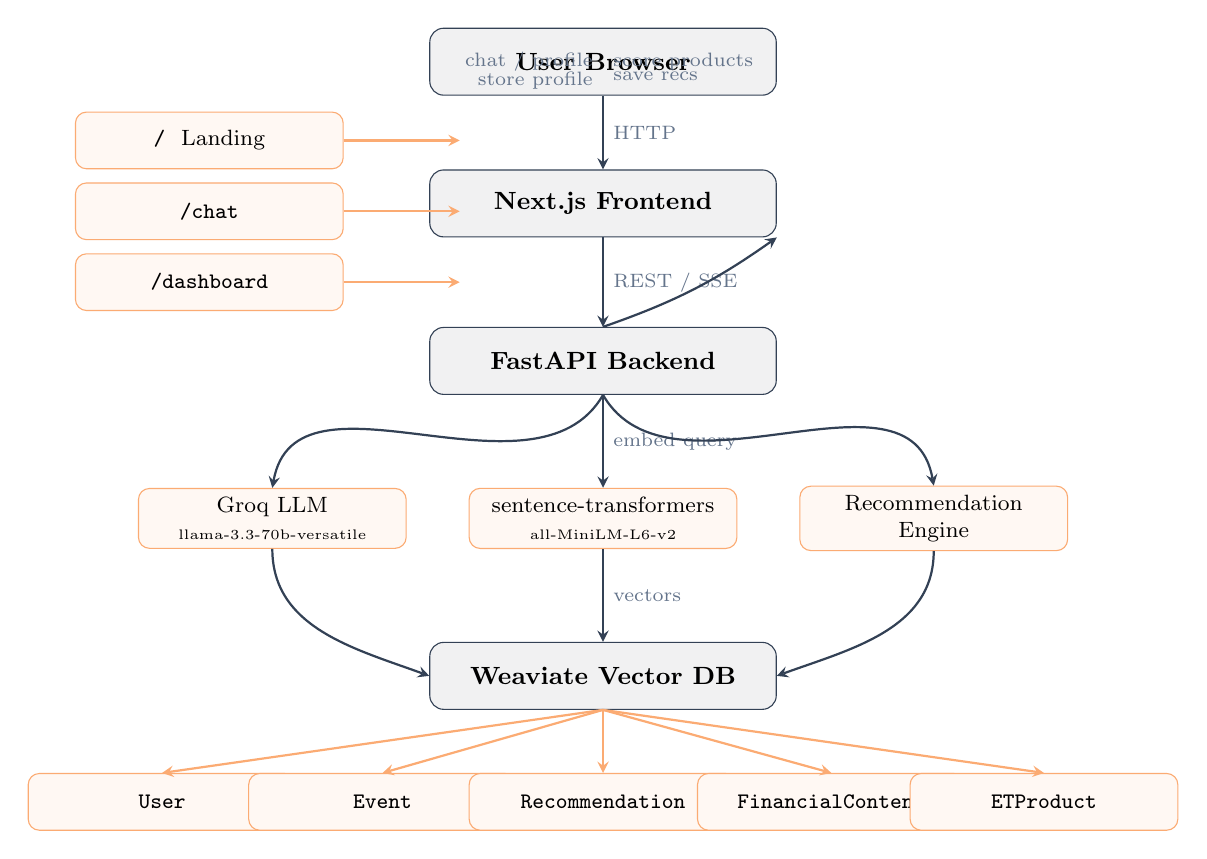
\begin{tikzpicture}[
  box/.style={
    draw=etSlate, rounded corners=5pt,
    fill=etDark!6, minimum width=4.4cm, minimum height=0.85cm,
    align=center, font=\small\bfseries
  },
  sbox/.style={
    draw=etOrange!60, rounded corners=4pt,
    fill=etOrange!5, minimum width=3.4cm, minimum height=0.72cm,
    align=center, font=\footnotesize
  },
  arr/.style={->, thick, color=etSlate, >=stealth},
  larr/.style={->, thick, color=etOrange!60, >=stealth},
]

%% Layer 1 — User
\node[box] (user)    at (0, 0)    {User Browser};

%% Layer 2 — Frontend
\node[box] (nextjs)  at (0, -1.8) {Next.js Frontend};
\node[sbox] (pg1)    at (-5.0, -1.0) {\texttt{/} \ Landing};
\node[sbox] (pg2)    at (-5.0, -1.9) {\texttt{/chat}};
\node[sbox] (pg3)    at (-5.0, -2.8) {\texttt{/dashboard}};

%% Layer 3 — Backend
\node[box] (fastapi) at (0, -3.8) {FastAPI Backend};

%% Layer 4 — Services
\node[sbox] (groq)   at (-4.2, -5.8) {Groq LLM\\{\tiny llama-3.3-70b-versatile}};
\node[sbox] (embed)  at (0,    -5.8) {sentence-transformers\\{\tiny all-MiniLM-L6-v2}};
\node[sbox] (reco)   at (4.2,  -5.8) {Recommendation\\Engine};

%% Layer 5 — Weaviate
\node[box] (weaviate) at (0, -7.8) {Weaviate Vector DB};

%% Layer 6 — Collections
\node[sbox] (c1) at (-5.6, -9.4) {\texttt{User}};
\node[sbox] (c2) at (-2.8, -9.4) {\texttt{Event}};
\node[sbox] (c3) at (0,    -9.4) {\texttt{Recommendation}};
\node[sbox] (c4) at (2.9,  -9.4) {\texttt{FinancialContent}};
\node[sbox] (c5) at (5.6,  -9.4) {\texttt{ETProduct}};

%% ── Arrows ────────────────────────────────────────────────────────────────

% User ↔ Frontend
\draw[arr] (user.south) -- (nextjs.north)
  node[midway, right, font=\scriptsize, text=etMuted] {HTTP};

% Frontend sub-pages (left panel)
\draw[larr] (pg1.east) -- (-1.82, -1.0);
\draw[larr] (pg2.east) -- (-1.82, -1.9);
\draw[larr] (pg3.east) -- (-1.82, -2.8);

% Frontend ↔ Backend
\draw[arr] (nextjs.south) -- (fastapi.north)
  node[midway, right, font=\scriptsize, text=etMuted] {REST / SSE};
\draw[arr] (fastapi.north) to[bend right=8] (nextjs.south east);

% Backend → Services
\draw[arr] (fastapi.south) to[out=240, in=80]  (groq.north)
  node[pos=0.45, left, font=\scriptsize, text=etMuted] {chat / profile};
\draw[arr] (fastapi.south) -- (embed.north)
  node[midway, right, font=\scriptsize, text=etMuted] {embed query};
\draw[arr] (fastapi.south) to[out=300, in=100] (reco.north)
  node[pos=0.45, right, font=\scriptsize, text=etMuted] {score products};

% Services → Weaviate
\draw[arr] (groq.south)  to[out=270, in=160] (weaviate.west)
  node[pos=0.6, below left, font=\scriptsize, text=etMuted] {store profile};
\draw[arr] (embed.south) -- (weaviate.north)
  node[midway, right, font=\scriptsize, text=etMuted] {vectors};
\draw[arr] (reco.south)  to[out=270, in=20]  (weaviate.east)
  node[pos=0.6, below right, font=\scriptsize, text=etMuted] {save recs};

% Weaviate → Collections
\foreach \c in {c1,c2,c3,c4,c5}{
  \draw[larr] (weaviate.south) -- (\c.north);
}

\end{tikzpicture}
\end{center}

% ══════════════════════════════════════════════════════════════════════════════
\section{Technology Stack}

\begin{table}[H]
\centering
\caption{Technology Stack Summary}
\begin{tabularx}{\textwidth}{llX}
\toprule
\textbf{Layer} & \textbf{Technology} & \textbf{Rationale} \\
\midrule
Frontend & Next.js 14 (App Router) & SSR, streaming support, TypeScript \\
Styling & Tailwind CSS + Framer Motion & Dark glassmorphism UI, micro-animations \\
Backend & FastAPI (Python 3.11) & Async, modular routers, auto-generated API docs \\
LLM & Groq \texttt{llama-3.3-70b-versatile} & Free tier, 6000 tokens/min, low latency \\
Vector DB & Weaviate (Cloud + local Docker) & Vector search + structured storage in one \\
Embeddings & \texttt{all-MiniLM-L6-v2} & 80MB, local, no API cost, excellent quality \\
\bottomrule
\end{tabularx}
\end{table}

% ══════════════════════════════════════════════════════════════════════════════
\section{Database Design}

All data is stored in Weaviate. We use five collections:

\begin{table}[H]
\centering
\caption{Weaviate Collection Schema}
\begin{tabularx}{\textwidth}{llX}
\toprule
\textbf{Collection} & \textbf{Vectorized} & \textbf{Fields} \\
\midrule
\texttt{User} & No & name, persona, risk\_level, goals, interests, recommended\_products, created\_at \\
\texttt{Event} & No & user\_id, event\_type (click/search/view), metadata (JSON), timestamp \\
\texttt{Recommendation} & No & user\_id, product, reason, score, created\_at \\
\texttt{FinancialContent} & \textbf{Yes} & title, content, category, tags \\
\texttt{ETProduct} & \textbf{Yes} & name, category, description, target\_persona, risk\_level, url \\
\bottomrule
\end{tabularx}
\end{table}

Collections marked as \textit{Vectorized} use \texttt{near\_vector} queries for semantic similarity search in the RAG pipeline.

% ══════════════════════════════════════════════════════════════════════════════
\section{API Reference}

\begin{table}[H]
\centering
\caption{REST API Endpoints}
\begin{tabularx}{\textwidth}{llX}
\toprule
\textbf{Method} & \textbf{Endpoint} & \textbf{Description} \\
\midrule
POST & \texttt{/chat} & Main conversational endpoint (onboarding + RAG) \\
POST & \texttt{/chat/stream} & SSE streaming for real-time typing effect \\
POST & \texttt{/profile/init} & Manually create a user profile \\
GET  & \texttt{/profile/\{user\_id\}} & Retrieve user profile \\
POST & \texttt{/events} & Log a user behaviour event \\
GET  & \texttt{/recommendations} & Get stored recommendations for user \\
POST & \texttt{/recommendations/refresh} & Re-score recommendations using latest events \\
GET  & \texttt{/user/\{user\_id\}} & Retrieve full user data \\
\bottomrule
\end{tabularx}
\end{table}

% ══════════════════════════════════════════════════════════════════════════════
\section{LLM Prompt Engineering}

\subsection{Onboarding System Prompt}
The concierge prompt is carefully engineered to:
\begin{itemize}[noitemsep]
  \item Ask \textbf{one question at a time} to avoid overwhelming the user
  \item Cover seven key profiling areas (name, occupation, goals, investments, risk, needs, ET familiarity)
  \item Signal completion with a consistent phrase for programmatic detection
  \item Stay under 80 words per response to maintain engagement
\end{itemize}

\subsection{Profile Extraction Prompt}
The extraction prompt uses \textbf{temperature = 0.1} (near-deterministic) to ensure reliable JSON output. It:
\begin{itemize}[noitemsep]
  \item Receives the full conversation transcript
  \item Returns a strict JSON schema with five fields
  \item Strips markdown code fences automatically
  \item Has a retry mechanism if the first parse fails
\end{itemize}

\subsection{RAG Answer Prompt}
The RAG prompt:
\begin{itemize}[noitemsep]
  \item Uses at most 4 context chunks to stay token-efficient (\textless 2000 tokens input)
  \item Injects the user persona and risk level as a ``profile hint''
  \item Instructs the model to be concise (\textless 150 words) and practical
\end{itemize}

% ══════════════════════════════════════════════════════════════════════════════
\section{Frontend Design}

The frontend follows a dark glassmorphism aesthetic consistent with ET's premium brand identity:

\begin{table}[H]
\centering
\caption{Frontend Pages}
\begin{tabularx}{\textwidth}{llX}
\toprule
\textbf{Route} & \textbf{Page} & \textbf{Key Features} \\
\midrule
\texttt{/} & Landing Page & Hero section, stats, feature grid, CTA — animated with Framer Motion \\
\texttt{/chat} & AI Concierge & Real-time chat with typing indicator, SSE support, profile completion badge \\
\texttt{/dashboard} & Dashboard & Profile card, recommendation cards with score bars and ET product links \\
\bottomrule
\end{tabularx}
\end{table}

Key design decisions:
\begin{itemize}[noitemsep]
  \item \textbf{Stateless chat}: full message history sent on every request — no server-side session management
  \item \textbf{localStorage persistence}: \texttt{user\_id} is stored client-side for session continuity across page refreshes
  \item \textbf{Streaming support}: \texttt{/chat/stream} SSE endpoint enables character-by-character response rendering
\end{itemize}

% ══════════════════════════════════════════════════════════════════════════════
\section{Knowledge Base Seeding}

The system is pre-seeded with a curated knowledge base:

\begin{table}[H]
\centering
\caption{Seeded Knowledge Base}
\begin{tabularx}{\textwidth}{llX}
\toprule
\textbf{Type} & \textbf{Count} & \textbf{Topics} \\
\midrule
Financial Articles & 10 & SIP, mutual funds, ELSS, NPS, insurance, stocks, FDs, gold, emergency funds, credit scores \\
ET Products & 8 & ET Money SIP, ET Markets, Tax Saver ELSS, Term Insurance, FD, Personal Loan, Credit Card, NPS \\
\bottomrule
\end{tabularx}
\end{table}

Each article and product is embedded using \texttt{all-MiniLM-L6-v2} and stored in Weaviate with its vector representation, enabling semantic search queries.

% ══════════════════════════════════════════════════════════════════════════════
\section{Setup \& Deployment}

\subsection{Prerequisites}
\begin{itemize}[noitemsep]
  \item Python 3.11+, Node.js 18+
  \item Free accounts: \href{https://console.groq.com}{Groq} and \href{https://console.weaviate.cloud}{Weaviate Cloud}
\end{itemize}

\subsection{Installation}

\begin{lstlisting}[language=bash, caption=Backend Setup]
git clone https://github.com/nimish1402/ET-Concierge.git
cd ET-Concierge/backend
python -m venv venv && venv\Scripts\activate
pip install -r requirements.txt
copy .env.example .env   # fill in API keys
python utils/seed_data.py
uvicorn main:app --reload --port 8000
\end{lstlisting}

\begin{lstlisting}[language=bash, caption=Frontend Setup]
cd ET-Concierge/frontend
npm install
npm run dev
# Visit http://localhost:3000
\end{lstlisting}

% ══════════════════════════════════════════════════════════════════════════════
\section{Innovation Highlights}

\begin{highlight}
\textbf{What makes this solution stand out:}
\begin{enumerate}[noitemsep]
  \item \textbf{Zero paid APIs} — Groq free tier + Weaviate sandbox + local embeddings
  \item \textbf{Weaviate-only storage} — single database for both vector search and structured data, eliminating operational complexity
  \item \textbf{Self-completing onboarding} — the LLM autonomously decides when it has enough information, no rigid Q\&A script
  \item \textbf{Behaviour-driven scoring} — recommendations dynamically improve as the user interacts with the platform
  \item \textbf{Full SSE streaming} — real-time response rendering for premium UX, no polling needed
\end{enumerate}
\end{highlight}

% ══════════════════════════════════════════════════════════════════════════════
\section{Conclusion}

The ET AI Concierge successfully addresses all four problem statement components:

\begin{itemize}[noitemsep]
  \item[\checkmark] \textbf{ET Welcome Concierge} — 3-minute profiling chat with automatic persona extraction
  \item[\checkmark] \textbf{Financial Life Navigator} — RAG-powered Q\&A personalised to user profile
  \item[\checkmark] \textbf{Cross-Sell Engine} — behaviour-weighted scoring with real-time recalculation
  \item[\checkmark] \textbf{Services Marketplace Agent} — semantic search over ET's full product catalog
\end{itemize}

The platform is production-ready, cost-free to operate at small scale, and built on a modular architecture that can be extended with additional ET data sources, user segments, or LLM providers.

\vspace{1em}
\begin{center}
\textcolor{etMuted}{\rule{8cm}{0.4pt}}\\
\small\textcolor{etMuted}{Built with Groq · Weaviate · FastAPI · Next.js}
\end{center}

\end{document}
